\documentclass[11pt,a4paper]{article}

\usepackage[T1]{fontenc}
\usepackage{lmodern}
\usepackage{textcomp}
\usepackage{microtype}
\usepackage[a4paper,margin=2.35cm]{geometry}
\usepackage{amsmath,amssymb,bm}
\usepackage{array}
\usepackage{booktabs}
\usepackage{siunitx}
\usepackage{graphicx}
\usepackage{subcaption}
\usepackage{placeins}
\usepackage[numbers,sort&compress]{natbib}
\usepackage{xcolor}
\usepackage{hyperref}
\usepackage[nameinlink,noabbrev]{cleveref}

\hypersetup{
  colorlinks=true,
  linkcolor=blue!45!black,
  citecolor=blue!45!black,
  urlcolor=blue!45!black,
  pdftitle={Biexciton Binding and Radiative Lifetimes in Strongly Oblate Semi-Ellipsoidal Quantum Dots},
  pdfauthor={D. G. Gevorgyan and E. M. Kazaryan}
}

\graphicspath{{figures/}}
\sisetup{
  separate-uncertainty=true,
  detect-all,
  range-phrase=--,
  range-units=single
}

\newcommand{\EX}{E_X}
\newcommand{\EXX}{E_{XX}}
\newcommand{\Ebind}{E_{\mathrm{bind}}}
\newcommand{\tauX}{\tau_X}
\newcommand{\tauXX}{\tau_{XX}}
\newcommand{\MX}{M_X}
\newcommand{\NX}{N_X}
\newcommand{\rB}{r_{\mathrm B}}
\newcommand{\Ry}{\mathrm{Ry}}
\newcommand{\meff}{m_e}
\newcommand{\mheff}{m_h}
\newcommand{\dd}{\mathop{}\!\mathrm{d}}
\newcommand{\vect}[1]{\bm{#1}}

\DeclareMathOperator{\Var}{Var}

\crefname{equation}{Eq.}{Eqs.}
\Crefname{equation}{Equation}{Equations}
\crefname{figure}{Fig.}{Figs.}
\Crefname{figure}{Figure}{Figures}
\crefname{table}{Table}{Tables}
\Crefname{table}{Table}{Tables}


\title{\textbf{Biexciton Binding and Radiative Lifetimes in Strongly Oblate
Semi-Ellipsoidal Quantum Dots}}
\author{D. G. Gevorgyan, E. M. Kazaryan\\
\small Russian-Armenian University\\
\small Corresponding author: \href{mailto:davitgevorgyan2000@gmail.com}{davitgevorgyan2000@gmail.com}}
\date{}

\begin{document}

\maketitle
\begin{abstract}
We investigate the ground exciton and biexciton states in a hard-wall,
strongly oblate semi-ellipsoidal GaAs quantum dot. Their energies are evaluated
variationally using correlated trial states constructed from analytical
single-particle wave functions, together with a ground-orbital-matched
importance transformation and adaptive quasi-Monte Carlo integration. A
noise-aware coordinate pattern search with two-budget verification is used to optimize
the variational parameters along intersecting axial and lateral geometry
scans. Because the effective-mass hard-wall model is intended to isolate
geometrical effects, the principal results are qualitative trends rather than
absolute predictions for a particular fabricated dot. The axial dimension
controls the absolute confinement energy much more strongly than the lateral
dimension, whereas enlargement along either direction weakens the biexciton
binding. The central binding estimate remains positive throughout the sampled
range but is not resolved from zero at the widest lateral geometry. Increasing
either semiaxis enhances the exciton coincidence overlap and oscillator
strength and therefore shortens the calculated radiative lifetimes. The
lateral dependence remains pronounced where the axial dependence approaches
saturation. These results distinguish the dominant axial control of the
confinement-energy scale from the important lateral control of weak
biexciton binding and radiative strength.
\end{abstract}

\noindent\textbf{Keywords:} semi-ellipsoidal quantum dot; exciton;
biexciton; binding energy; variational method; quasi-Monte Carlo integration;
radiative lifetime


\section{Introduction}
\label{sec:introduction}

Semiconductor quantum dots provide discrete, atom-like carrier spectra while
retaining substantial control through composition, confinement, and external
geometry. Their neutral exciton ($X$) and biexciton ($XX$) states form the
elementary ladder for correlated photon emission. In particular, the
biexciton--exciton cascade has enabled regulated photon-pair emission
\cite{benson2000,moreau2001} and polarization-entangled photon generation
\cite{akopian2006}. The biexciton binding energy determines the separation of
the two cascade transitions and therefore affects spectral addressability,
resonant excitation, and regimes in which the emitted photons approach equal
energies.

The energy of a confined biexciton is not fixed by a single Coulomb scale.
Electron--hole attraction competes with electron--electron and hole--hole
repulsion, while the carrier masses and the confinement geometry determine how
strongly the four particles can rearrange. Consequently, biexcitons may be
bound, antibound, or close to zero binding even within the same material
system. Experimental studies have likewise shown that biexciton binding can
change strongly with confinement and dot structure
\cite{bayer1998,juska2019}. This sensitivity makes the biexciton a useful
probe of few-particle correlations, but it also makes its numerical evaluation
demanding: the binding energy is a small difference between two much larger
correlated energies.

Strongly oblate quantum dots are especially suitable for separating the roles
of axial and lateral confinement. Their two semiaxes provide independent
geometrical controls, while the large separation between axial and in-plane
energy scales permits an adiabatic treatment of the single-particle states.
Variational calculations for strongly oblate ellipsoidal dots have demonstrated
geometry-dependent energies, binding energies, recombination energies, and
radiative lifetimes \cite{hayrapetyan2019}, and subsequent work extended the
same framework to nonlinear optical response \cite{bleyan2022}. The
semi-ellipsoidal boundary considered here is relevant to flattened or
dome-like dots and has previously been used for single-particle and interband
absorption calculations \cite{hayrapetyan2012}. Unlike a full ellipsoid, the
dot occupies only one side of the basal plane, which changes the axial
boundary condition while retaining axial rotational symmetry.

The purpose of this work is to determine how the lateral semiaxis $a$ and
axial semiaxis $c$ control the corrected energy, binding, and radiative
lifetime of the biexciton in a strongly oblate
semi-ellipsoidal GaAs dot. We restrict the study to the single-particle ground
configuration and use correlated variational states for both $X$ and $XX$.
The high-dimensional integrals are evaluated after a state-matched importance
transformation. For the final biexciton calculation we retain the full
symmetrized correlation expression and remove only the redundant global
rotation, thereby avoiding the accumulation of independent quadrature errors
among analytically equivalent reduced terms. The variational parameters are
then refined by a safeguarded coordinate pattern search that verifies accepted
moves at two integration budgets.

Seven geometries form two intersecting scans: $c=0.5,1,1.5,2$ at fixed
$a=5$, and $a=3,5,7,10$ at fixed $c=1$, with all lengths measured in the
effective electron Bohr radius. From the optimized states we obtain $\EX$,
$\EXX$, $\Ebind=2\EX-\EXX$, the exciton coincidence overlap, and the
radiative lifetimes $\tauX$ and $\tauXX$. Particular attention is paid to the
numerical resolution of the small binding energy. The reported error bars are
rough propagations of the adaptive integrator's internal estimates rather than
formal statistical confidence intervals.

\section{Model and theoretical framework}
\label{sec:theory}

The interacting exciton and biexciton ground-state energies are obtained with
the variational method: trial correlation factors are optimized by minimizing
the corresponding Hamiltonian expectation values. We first establish the
single-particle confinement states on which these trial states are built.

\subsection{Geometry, units, and single-particle ground state}
\label{sec:single-particle}

We consider a hard-wall semi-ellipsoidal quantum dot with cylindrical
coordinates $\vect r=(r,\phi,z)$ and confinement potential
\begin{equation}
 V_{\mathrm{conf}}(r,z)=
 \begin{cases}
  0, & r^2/a^2+z^2/c^2\leq 1\ \text{and}\ z\geq0,\\
  \infty, & \text{otherwise},
 \end{cases}
 \qquad c/a\ll1 .
 \label{eq:confinement-potential}
\end{equation}
The in-plane and axial semiaxes are $a$ and $c$, respectively, as illustrated
in \cref{fig:semi-ellipsoid}.

\begin{figure}[ht]
 \centering
 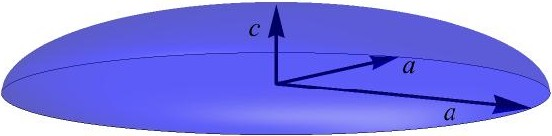
\includegraphics[width=0.52\linewidth]{Semi-ellipsoid.jpeg}
 \caption{Semi-ellipsoidal quantum-dot geometry, with lateral semiaxis $a$
 and axial semiaxis $c$.}
 \label{fig:semi-ellipsoid}
\end{figure}

Lengths and energies are expressed in the effective electron Bohr radius and
Rydberg,
\begin{equation}
 \rB=\frac{4\pi\epsilon_0\epsilon_r^{(E)}\hbar^2}{\meff e^2},
 \qquad
 E_{\mathrm R}=\frac{\hbar^2}{2\meff\rB^2}.
 \label{eq:effective-units}
\end{equation}
For the GaAs energy calculation we use the standard bulk parameter set
\cite{vurgaftman2001},
$\epsilon_r^{(E)}=12.8$, $\meff=0.067m_0$, and
$\mheff=0.45m_0$, giving
$\rB=\SI{10.109654}{nm}$ and
$E_{\mathrm R}=\SI{5.563851565}{meV}$.

Because the axial confinement is much stronger than the in-plane
confinement, the single-particle problem is treated adiabatically
\cite{hayrapetyan2012}. At fixed $r$, the available height is
\begin{equation}
 z_{\max}(r)=c\sqrt{1-r^2/a^2},
 \label{eq:zmax}
\end{equation}
and the lowest axial factor is
\begin{equation}
 \chi_1(z;r)=
 \sqrt{\frac{2}{z_{\max}(r)}}
 \sin\left[\frac{\pi z}{z_{\max}(r)}\right].
 \label{eq:axial-wavefunction}
\end{equation}
For a carrier of mass $m_q$ with $q=e,h$ the axial eigenenergy acts as the adiabatic
potential for the slow planar motion,
\begin{equation}
 U_q(r)=\frac{\meff}{m_q}\frac{\pi^2}{z_{\max}^2(r)}
 =\frac{\meff}{m_q}\frac{\pi^2}{c^2}
   \left(1+\frac{r^2}{a^2}+O(r^4/a^4)\right),
 \label{eq:adiabatic-potential}
\end{equation}
where lengths and energies are in the effective units of
\cref{eq:effective-units}. Thus, after subtracting the constant axial energy,
the planar harmonic-oscillator Hamiltonian is
\begin{equation}
 H_{q,\parallel}=\frac{\meff}{m_q}
 \left[-\nabla_{\parallel}^2+\frac{\pi^2r^2}{a^2c^2}\right].
 \label{eq:planar-hamiltonian}
\end{equation}
Writing $\lambda=\pi/(ac)$, its normalized ground-state component and the
corresponding axial and planar ground-state energies are
\begin{equation}
 \varphi_{q,\parallel}(r)=\sqrt{\frac{\lambda}{\pi}}
 e^{-\lambda r^2/2},\qquad
 \varepsilon_{q,z}=\frac{\meff}{m_q}\frac{\pi^2}{c^2},\qquad
 \varepsilon_{q,\parallel}=\frac{\meff}{m_q}\frac{2\pi}{ac}.
 \label{eq:single-particle-scales}
\end{equation}
The total ground-state confinement energy of carrier $q$ is therefore
\begin{equation}
 E_q=\varepsilon_{q,z}+\varepsilon_{q,\parallel}
 =\frac{\meff}{m_q}\left(\frac{\pi^2}{c^2}+\frac{2\pi}{ac}\right).
 \label{eq:carrier-ground-energy}
\end{equation}
The normalized carrier ground orbital is therefore
$\psi_q(r,\phi,z)=\chi_1(z;r)\varphi_{q,\parallel}(r)$. Thus the uncorrelated exciton and biexciton confinement energies are
\begin{equation}
 E_X^{(0)}=E_e+E_h,\qquad
 E_{XX}^{(0)}=2E_e+2E_h=2E_X^{(0)}.
 \label{eq:single-particle-energies}
\end{equation}
The band gap is not included in these energies.

\subsection{Correlated exciton}
\label{sec:exciton-model}

We denote electron coordinates by $1,2$ and hole coordinates by $a,b$; the
ground exciton uses coordinates $1$ and $a$. Pair distances are the
three-dimensional Euclidean distances $r_{ij}=|\vect r_i-\vect r_j|$. In the
effective units of \cref{eq:effective-units}, its Hamiltonian is
\begin{equation}
 H_X=h_e(1)+h_h(a)-\frac{2}{r_{1a}},
 \qquad
 h_e\psi_e=E_e\psi_e,\quad h_h\psi_h=E_h\psi_h.
 \label{eq:exciton-hamiltonian}
\end{equation}
The uncorrelated state $\Psi_{0X}=\psi_e(1)\psi_h(a)$ is therefore an
eigenstate of $h_e+h_h$ with energy $E_X^{(0)}=E_e+E_h$. Electron--hole
correlation is introduced through
\begin{equation}
 \Psi_X=\Psi_{0X}F_X,\qquad F_X=\exp(-\alpha_X r_{1a}),
 \label{eq:exciton-trial}
\end{equation}
where $\alpha_X>0$ is varied independently at each geometry. The variational
energy is evaluated from
\begin{equation}
 E_X=\frac{\langle\Psi_X|H_X|\Psi_X\rangle}
 {\langle\Psi_X|\Psi_X\rangle}.
 \label{eq:exciton-expectation}
\end{equation}
The denominator is
\begin{equation}
 \NX=\int
 |\Psi_{0X}|^2F_X^2\dd\tau
 =\int|\Psi_{0X}|^2e^{-2\alpha_X r_{1a}}\dd\tau .
 \label{eq:exciton-norm}
\end{equation}
Using the single-particle eigenvalue equations in
\cref{eq:exciton-hamiltonian} and integrating the kinetic terms by parts gives
\begin{equation}
 E_X=E_X^{(0)}+\frac{1}{\NX}\int|\Psi_{0X}|^2
 \left[|\nabla_1F_X|^2+\frac{\meff}{\mheff}|\nabla_aF_X|^2
 -\frac{2F_X^2}{r_{1a}}\right]\dd\tau .
 \label{eq:exciton-energy-integral}
\end{equation}
Since $|\nabla_1r_{1a}|=|\nabla_ar_{1a}|=1$, the kinetic contribution
generated by $F_X$ is
\begin{equation}
 K_X(\alpha_X)=
 \alpha_X^2\left(1+\frac{\meff}{\mheff}\right).
 \label{eq:exciton-kinetic}
\end{equation}
Defining the Coulomb numerator as
\begin{equation}
 V_X=\int
 |\Psi_{0X}|^2F_X^2
 \left(-\frac{2}{r_{1a}}\right)\dd\tau
 \label{eq:exciton-coulomb}
\end{equation}
reduces \cref{eq:exciton-energy-integral} to
\begin{equation}
 \EX=E_X^{(0)}+\Delta E_X,\qquad
 \Delta E_X=K_X+\frac{V_X}{\NX}.
 \label{eq:exciton-energy}
\end{equation}
For each dot geometry, the remaining integrals $N_X$ and $V_X$ are evaluated
numerically.

\subsection{Correlated biexciton}
\label{sec:biexciton-model}

The two-electron--two-hole interaction in effective units is
\begin{equation}
 V_{XX}=2\left(
 \frac{1}{r_{12}}+\frac{1}{r_{ab}}
 -\frac{1}{r_{1a}}-\frac{1}{r_{1b}}
 -\frac{1}{r_{2a}}-\frac{1}{r_{2b}}
 \right).
 \label{eq:biexciton-coulomb}
\end{equation}
For the biexciton we use the ansatz~\cite{}
\begin{equation}
 \Psi_{XX}=\Psi_{0XX}F_{XX},\qquad
 \Psi_{0XX}=\psi_e(1)\psi_e(2)\psi_h(a)\psi_h(b),
 \label{eq:biexciton-trial}
\end{equation}
with the exchange-symmetric correlation factor
\begin{equation}
\begin{aligned}
 F_{XX}&=G(P+Q),\\
 G&=r_{ab}^{\gamma}e^{-\delta r_{ab}},\\
 P&=\exp\left[-\alpha(r_{1a}+r_{2b})
                 -\beta(r_{1b}+r_{2a})\right],\\
 Q&=\exp\left[-\beta(r_{1a}+r_{2b})
                 -\alpha(r_{1b}+r_{2a})\right].
\end{aligned}
 \label{eq:correlation-factor}
\end{equation}
The four variational parameters $(\alpha,\beta,\gamma,\delta)$ control the
direct and cross electron--hole pairings and the hole--hole correlation.

To write the kinetic numerator compactly, define
$\vect g_i^P=\nabla_i\ln(GP)$ and
$\vect g_i^Q=\nabla_i\ln(GQ)$. For electron coordinates the derivatives of
$G$ vanish, whereas for hole coordinates they contain the logarithmic
derivative of $G$ in \cref{eq:correlation-factor}. Unlike the exciton kinetic contribution,
the biexciton kinetic numerator has no analytical form and is written as
\begin{equation}
 K_{XX}=\int|\Psi_{0XX}|^2G^2\left[\sum_{i=1,2}|P\vect g_i^P+Q\vect g_i^Q|^2+\frac{\meff}{\mheff}\sum_{j=a,b}|P\vect g_j^P+Q\vect g_j^Q|^2\right]\dd\tau .
 \label{eq:biexciton-kinetic-numerator}
\end{equation}
The energy is then
\begin{equation}
 \EXX=E_{XX}^{(0)}+\Delta E_{XX},\qquad
 \Delta E_{XX}=
 \frac{K_{XX}+\langle\Psi_{XX}|V_{XX}|\Psi_{XX}\rangle}
 {\langle\Psi_{XX}|\Psi_{XX}\rangle}.
 \label{eq:biexciton-energy}
\end{equation}
In the numerical calculation, the kinetic contribution in
\cref{eq:biexciton-kinetic-numerator} and the potential contribution are
combined and evaluated in a single integral. No direct/cross or
particle-exchange multiplicities are introduced in the final estimator.

We define the biexciton binding energy as
\begin{equation}
 \Ebind=2\EX-\EXX
       =2\Delta E_X-\Delta E_{XX}.
 \label{eq:binding-energy}
\end{equation}
With this convention $\Ebind>0$ denotes a bound biexciton. The
single-particle part cancels exactly, making \cref{eq:binding-energy} a small
difference of correlation corrections.

\subsection{Radiative lifetimes}
\label{sec:observables}

Following Hayrapetyan \textit{et al.}\ \cite{hayrapetyan2019}, we calculate the exciton and biexciton radiative lifetimes from
\begin{equation}
 \tauX=
 \frac{2\pi\epsilon_0\meff c_0^3\hbar^2}
 {\sqrt{\epsilon_r^{(\mathrm{opt})}}\,e^2
 E_{\mathrm{exc}}^2f_X},
 \qquad
 \tauXX=\frac{\tauX}{4}.
 \label{eq:lifetimes}
\end{equation}
The relation $\tauXX=\tauX/4$ follows the biexciton decay-channel convention
of Ref.~\cite{hayrapetyan2019}; it is not an independently optimized quantity.

Evaluation of $\tauX$ requires the oscillator strength and transition energy,
which are
\begin{equation}
 f_X=\frac{E_P}{E_{\mathrm{exc}}}|\MX|^2,\qquad
 E_{\mathrm{exc}}=E_g+\EX,
 \label{eq:oscillator-strength}
\end{equation}
where, $E_g$ is the band gap. The remaining quantity $\MX$ is the electron--hole coincidence overlap. At
coincidence the exciton Jastrow factor in \cref{eq:exciton-trial} is unity,
and because the electron and hole ground orbitals are matched in the present
model, the normalized overlap reduces to
\begin{equation}
 \MX=\frac{1}{\sqrt{\NX}},\qquad
 |\MX|^2=\frac{1}{\NX}.
 \label{eq:coincidence-overlap}
\end{equation}
Thus the lifetime can be obtained from the already calculated exciton norm;
no additional oscillator-strength integral is required.

For the optical calculation we take
$E_g=\SI{1.5192}{eV}$, $\meff=0.0665m_0$,
$E_P=\SI{22.71}{eV}$, and
$\epsilon_r^{(\mathrm{opt})}=12.91$, matching the parameter set of
Ref.~\cite{hayrapetyan2019}. We keep this optical set distinct from the bulk
parameters in \cref{eq:effective-units} because the latter define the units
and single-particle states used in the variational energy calculation,
whereas the former enter the dimensional radiative-lifetime parametrization.
This separation preserves the energy calculation while reproducing the
cited optical calibration.

\section{Numerical method and validation}
\label{sec:numerics}

\subsection{Geometry and integration parametrization}
\label{sec:importance}

We study the seven geometries listed in \cref{tab:geometries}. The common
point $(5,1)$ links a scan of axial confinement to a scan of lateral
confinement.

\begin{table}[ht]
 \centering
 \caption{Quantum-dot semiaxes used in the axial and lateral scans, in
 effective Bohr radii.}
 \label{tab:geometries}
 \begin{tabular}{lcc}
  \toprule
  Scan & $a$ & $c$\\
  \midrule
  Axial & 5 & 0.5, 1, 1.5, 2\\
  Lateral & 3, 5, 7, 10 & 1\\
  \bottomrule
 \end{tabular}
\end{table}

Direct integration in the physical coordinates is inefficient because the
single-particle orbitals occupy only a small part of the nominal domain. We
therefore transform every particle to variables matched to the ground-state
density. The axial coordinate is first written
\begin{equation}
 z=u\,c\sqrt{1-r^2/a^2},\qquad 0<u<1 .
 \label{eq:axial-map}
\end{equation}
The numerical radial domain is restricted to the validated cutoff $R=0.9a$.
Using the ground-state in-plane length $\ell$, the reference radial and axial
densities are
\begin{equation}
 p_r(r)=\frac{1}{C}\frac{2r}{\ell^2}e^{-r^2/\ell^2},
 \quad C=1-e^{-R^2/\ell^2},
 \qquad
 p_u(u)=2\sin^2(\pi u).
 \label{eq:reference-densities}
\end{equation}
Both reference densities have analytical cumulative distributions. For the
radial density, the inverse is
\begin{equation}
 r(v)=\ell\sqrt{-\ln(1-Cv)},\qquad 0<v<1,
 \label{eq:radial-inverse}
\end{equation}
whereas the axial cumulative distribution has no elementary closed form inverse and is tabulated once and
interpolated. This transformation cancels most of the localized
single-particle density and leaves an order-unity transformed integrand. It is
an importance transformation, not a symmetry reduction.

The final estimator removes only the redundant global azimuthal rotation. For
the exciton, the hole angle is fixed to zero, the electron angle spans
$[0,2\pi]$, and a factor $2\pi$ restores the global rotation. For the
biexciton, $\phi_a=0$ while $\phi_1$, $\phi_2$, and $\phi_b$ are each
integrated independently over $[0,2\pi]$, again with an overall factor
$2\pi$. No reflection folding or particle-exchange multiplicities are used.
The complete $G(P+Q)$ factor, the six Coulomb interactions in
\cref{eq:biexciton-coulomb}, and the four kinetic contributions in
\cref{eq:biexciton-kinetic-numerator} remain in the pointwise integrand.

\subsection{Adaptive quasi-Monte Carlo quadrature}
\label{sec:quadrature}

Every integral is evaluated with the Wolfram Language implementation of
adaptive quasi-Monte Carlo quadrature. Low-discrepancy points improve the
coverage of the high-dimensional unit hypercube relative to independent
pseudorandom sampling \cite{caflisch1998}, while adaptive subdivision directs
additional evaluations toward regions with larger estimated error. The
production settings are
\begin{equation}
\begin{aligned}
 \texttt{Method}&=\texttt{AdaptiveQuasiMonteCarlo},\\
 \texttt{BisectionDithering}&=0,\\
 \texttt{AccuracyGoal}&=\infty,\qquad
 \texttt{PrecisionGoal}=4 .
\end{aligned}
\label{eq:qmc-settings}
\end{equation}
The stage-dependent point budget is supplied through
\texttt{MaxPoints}. A finite absolute accuracy goal is inappropriate because
some biexciton numerator and norm integrals are much smaller than a typical
absolute tolerance. Reaching \texttt{MaxPoints} therefore indicates that the
requested relative goal was not attained before the budget cap; the returned
integral value and internal error estimate are nevertheless retained.

The Hamiltonian numerator and norm denominator are independent adaptive calls.
They do not share a fixed Sobol point set. This preserves separate adaptation
to their different integrands. The internal quadrature errors returned for
the numerator and denominator are treated as independent and propagated to
the exciton and biexciton energies, the binding energy, and the radiative
lifetimes. The resulting error bars are numerical-resolution indicators, not
statistical confidence intervals: they neglect covariance between the
adaptive integrals, possible systematic quasi-Monte Carlo bias, and uncertainty
in the location of the variational optimum.

The final estimator was selected through a sequence of checks at $(5,1)$.
These included the exact exciton normalization at $\alpha_X=0$, integration
budget comparisons, dithered adaptive partitions, a complete four-angle
biexciton calculation, and the final global-rotation-fixed calculation. The
two angular formulations agree within the observed resolution, while removing
the redundant global angle reduces the numerical dimension. Earlier
direct/cross and particle-relabeling identities remain analytically valid,
but their independent numerical evaluations exhibited percent-level
differences and were therefore not used to assemble the final energies.

\subsection{Variational search}
\label{sec:optimization}

The variational search proceeded in two phases. The first was an exploratory
multidimensional search performed with the Wolfram Language function
\texttt{NMinimize} using the Nelder--Mead method. It varied the parameters
simultaneously at a lower integration budget and located approximate minima
for each geometry. Because small objective differences can be dominated by
quasi-Monte Carlo fluctuations, these first-phase optima were used only as
starting points.

The second phase refined those starting points with an automated local
coordinate pattern search using the integration setup of
\cref{sec:importance}. Positive and
negative displacements of each parameter were screened at a moderate budget;
the center and the most promising candidates were then recomputed at a larger
budget, with progressively smaller displacements used around stable
candidates. Automation generated and evaluated the candidates, but final
selection also relied on inspecting the energies, integration-error estimates,
stability between budgets, neighboring points in parameter space, and
consistency of the geometry trends. A parameter set was retained only when
this review indicated a stable local minimum rather than an isolated low
numerical fluctuation.

\section{Results and discussion}
\label{sec:results}

\subsection{Corrected exciton and biexciton energies}
\label{sec:energy-results}

The correlation corrections and corrected energies are collected in
\cref{tab:energies} of the Appendix. The results in
\cref{sec:energy-results,sec:binding-results,sec:overlap-results} are
dimensionless: lengths are scaled
by $\rB$ and energies by the effective Rydberg of
\cref{eq:effective-units}. At fixed effective-mass ratio
$\eta=\meff/\mheff$, they are material-scaled and do not require a dimensional
GaAs calibration. Conversion to dimensional units is used only for the
radiative-lifetime calculation. The values include the single-particle
confinement and correlation corrections but exclude the band gap. Because the
zeroth-order energies are analytical, each correlation correction has the
same numerical integration error as its corresponding corrected energy.
Although these rough errors are retained in the table, they are too small to
be visible on the scale of the biexciton-energy curves in \cref{fig:exx}.
The numerical values are reported for transparency and reproducibility, but
the physically relevant conclusions are the comparative geometry trends
within the idealized model rather than absolute predictions for a particular
quantum dot.

\begin{figure}[ht]
\centering
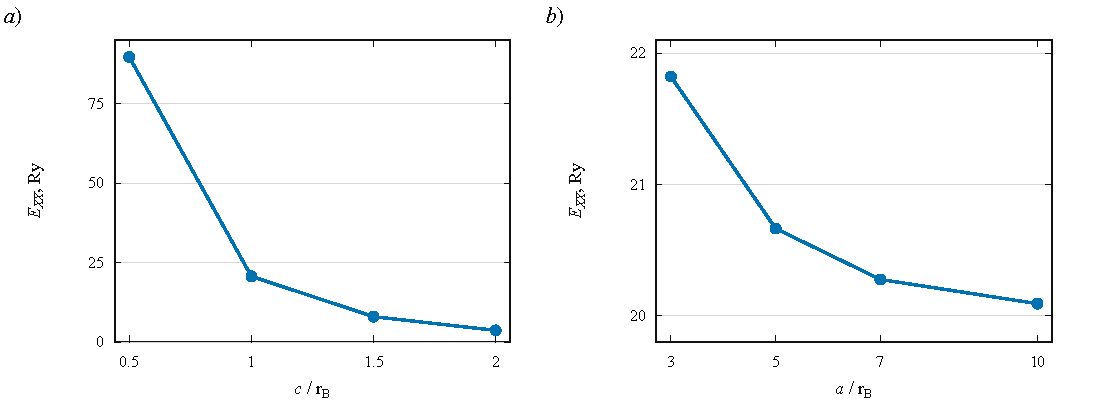
\includegraphics[width=\linewidth]{Main-E_XX-Ry.pdf}
\caption{Corrected biexciton energy as a function of
(a) the axial semiaxis $c$ at fixed $a=5\rB$ and (b) the lateral semiaxis
$a$ at fixed $c=\rB$, in effective Rydbergs. The band gap is excluded. Lines
are guides to the eye, and numerical error bars are smaller than the symbols
at the displayed scales.}
\label{fig:exx}
\end{figure}

Along the axial scan, $\EXX$ decreases steeply and nonlinearly, with most of
the change occurring between the two most strongly confined geometries. This
behavior reflects the strong sensitivity of the confinement energy to the
short semiaxis in the oblate regime.

The lateral scan is much flatter: enlarging the in-plane semiaxis produces
only a modest reduction in $\EXX$. The axial dimension is therefore the
dominant geometrical control of the absolute biexciton energy over the sampled
range, consistent with the separation of axial and lateral energy scales in
\cref{eq:single-particle-scales}.

\subsection{Biexciton binding}
\label{sec:binding-results}

\begin{figure}[ht]
\centering
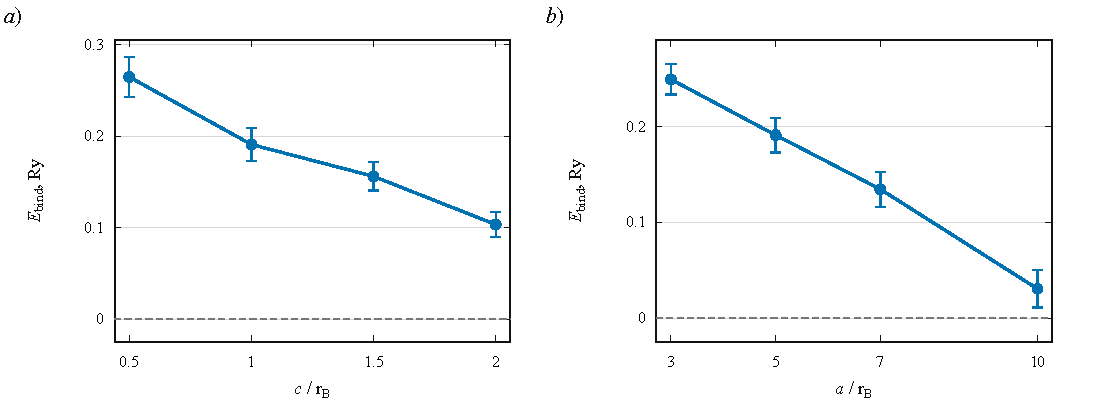
\includegraphics[width=\linewidth]{Main-Binding-Energy-Ry.pdf}
\caption{Binding energy $\Ebind=2\EX-\EXX$ as a function of (a) $c$ at
fixed $a=5\rB$ and (b) $a$ at fixed $c=\rB$, in effective Rydbergs. Positive
values correspond to a bound biexciton. The dashed line marks zero binding.
Error bars are rough first-order propagations of the adaptive-integration
estimates, not statistical confidence intervals.}
\label{fig:binding}
\end{figure}

The central binding energy is positive throughout the sampled geometries and
decreases monotonically when either semiaxis is increased
(\cref{fig:binding}). Thus relaxing axial or lateral confinement reduces the
net correlation advantage of the four-particle state relative to two isolated
excitons. The lateral scan approaches the zero-binding threshold more closely
than the axial scan.

The binding is well separated from zero at every geometry except the widest
lateral dot. There, the numerical-resolution estimate is comparable to the
small central binding energy. Because that estimate omits systematic
integration bias and uncertainty in the optimum, we classify the point as
marginally positive rather than claiming firmly resolved binding. No sign
change is demonstrated within the studied range.

Because the single-particle part cancels in \cref{eq:binding-energy}, the
origin of this trend is exposed by comparing the two correlation corrections
in \cref{fig:correlation-corrections}. Both become less negative as the dot is
enlarged, while the separation between $2\Delta E_X$ and $\Delta E_{XX}$
narrows. That separation is precisely $\Ebind$, so the convergence of the two
curves accounts directly for the suppression of binding, particularly along
the lateral scan.

\begin{figure}[ht]
\centering
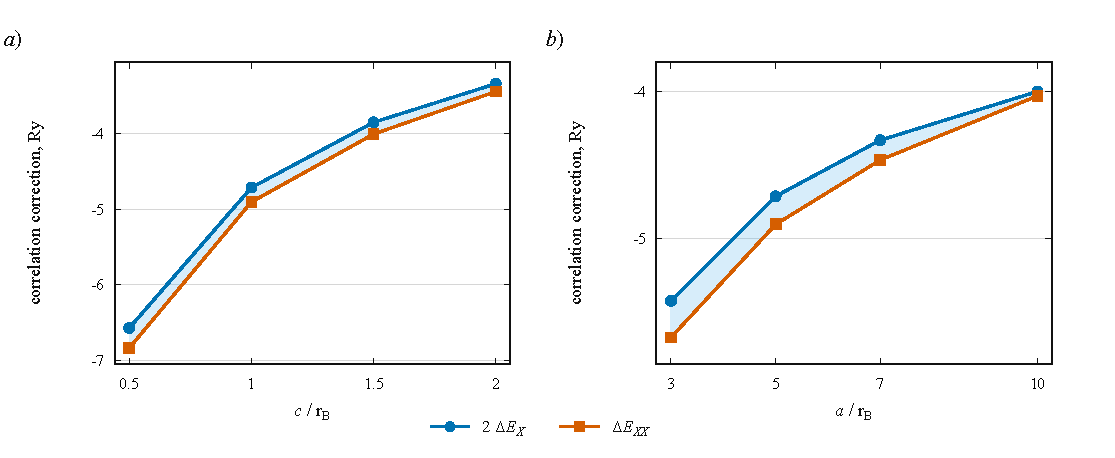
\includegraphics[width=\linewidth]{Main-Correlation-Corrections-Ry.pdf}
\caption{Comparison of the two-exciton correction $2\Delta E_X$ with the
biexciton correction $\Delta E_{XX}$ as functions of (a) $c$ at fixed
$a=5\rB$ and (b) $a$ at fixed $c=\rB$, in effective Rydbergs. Their vertical
separation equals the binding energy. Lines are guides to the eye; numerical
error bars are smaller than the plotted symbols at this scale.}
\label{fig:correlation-corrections}
\end{figure}

\FloatBarrier
\subsection{Variational parameters and optical intermediates}
\label{sec:overlap-results}

The complete optimized biexciton parameters are reported in
\cref{tab:parameters} of the Appendix and summarized graphically in
\cref{fig:parameters}. The exciton parameter $\alpha_X$ generally decreases along the
axial scan and increases along the lateral scan. For the biexciton, the
optimized cross-pair exponent $\beta$ becomes very small at the larger axial
sizes. The composite quantity $\gamma/\delta$, which sets the maximum of the isolated factor
$r_{ab}^{\gamma}e^{-\delta r_{ab}}$, increases smoothly as either dot
dimension is enlarged. This indicates that the hole--hole factor shifts
toward larger characteristic separations in larger dots.

\begin{figure}[ht]
\centering
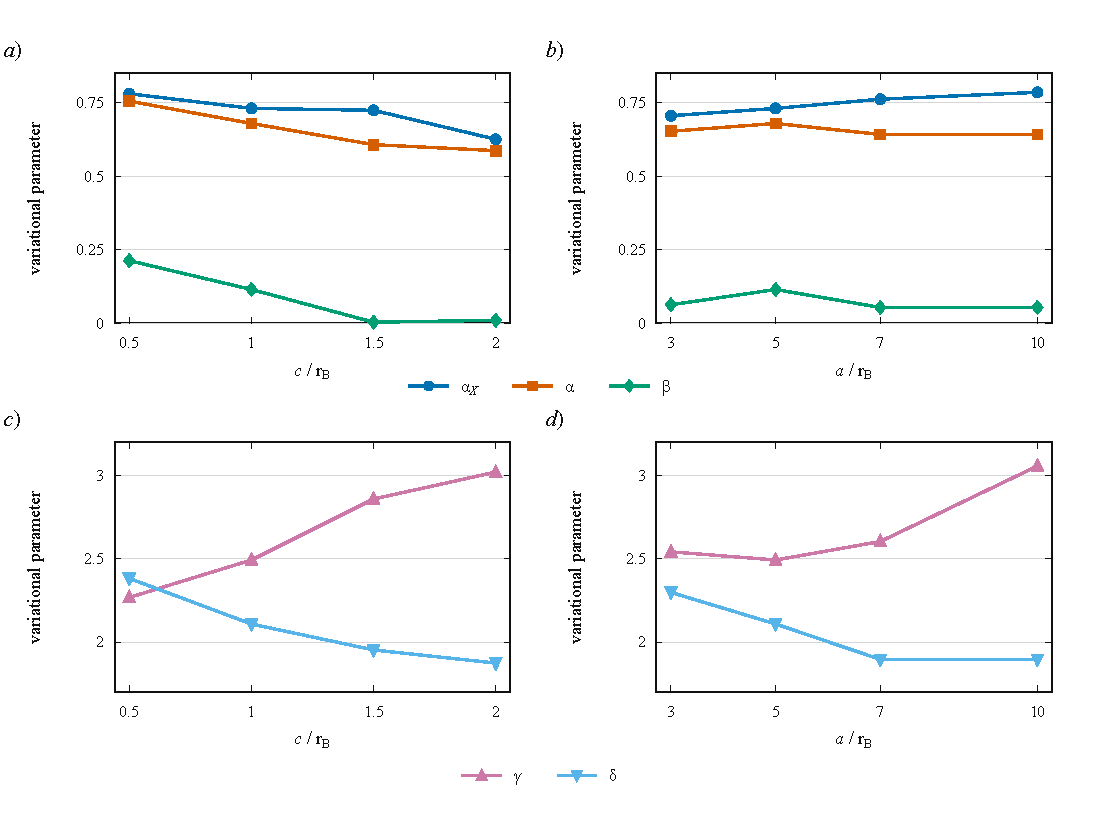
\includegraphics[width=\linewidth]{Main-Variational-Parameters.pdf}
\caption{Optimized variational parameters along the axial scan at fixed
$a=5\rB$ and the lateral scan at fixed $c=\rB$. Panels (a) and (b) show
$\alpha_X$, $\alpha$, and $\beta$; panels (c) and (d) show $\gamma$ and
$\delta$. Lines are guides to the eye.}
\label{fig:parameters}
\end{figure}

\FloatBarrier

These parameter-level trends should be interpreted more cautiously than the
energies. The objective is numerically rough, the second-phase search is local,
and different parameter combinations can produce energies separated by less
than the practical quadrature resolution. The parameters characterize the
retained variational minimum but are not claimed to be unique.

The coincidence overlap is shown in \cref{fig:overlap}, while the derived
optical quantities are listed in \cref{tab:optical} of the Appendix. The
overlap increases as either dot dimension is enlarged. It tends toward
saturation at the larger axial sizes, whereas it continues to rise across the
lateral scan. The oscillator strength follows the same behavior.

\begin{figure}[ht]
\centering
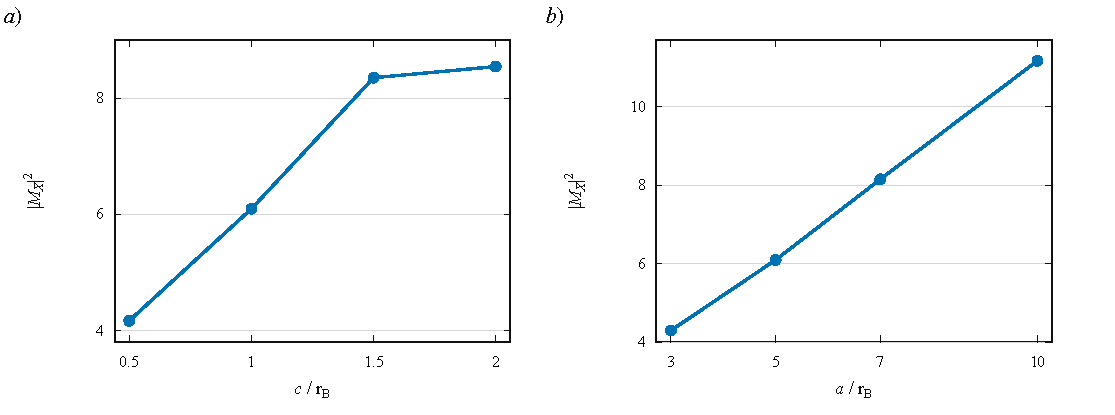
\includegraphics[width=\linewidth]{Main-Overlap.pdf}
\caption{Squared exciton coincidence overlap $|\MX|^2$ as a function of
(a) $c$ at fixed $a=5\rB$ and (b) $a$ at fixed $c=\rB$. Lines are guides to
the eye, and numerical error bars are smaller than the plotted symbols.}
\label{fig:overlap}
\end{figure}

\FloatBarrier

\FloatBarrier
\subsection{Radiative lifetimes}
\label{sec:lifetime-results}

\begin{figure}[ht]
\centering
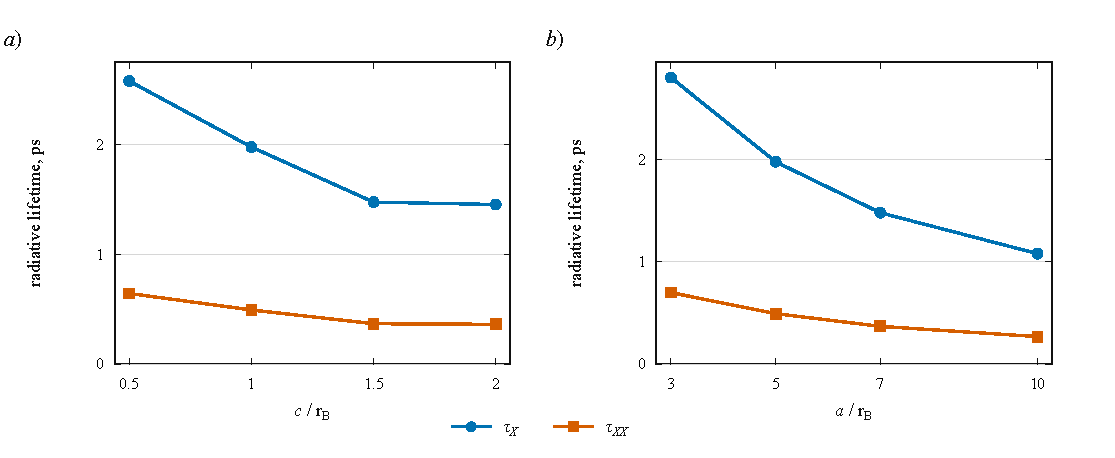
\includegraphics[width=\linewidth]{Main-Lifetimes.pdf}
\caption{Exciton and biexciton radiative lifetimes as functions of
(a) $c$ at fixed $a=5\rB$ and (b) $a$ at fixed $c=\rB$. The values use the
corrected optical transition energy and the coincidence overlap. The adopted
decay-channel convention gives $\tauXX=\tauX/4$. The single GaAs parameter
set is specified in \cref{sec:observables}. Propagated error bars are smaller
than the plotted symbols.}
\label{fig:lifetimes}
\end{figure}

Both radiative lifetimes decrease as the dot is enlarged
(\cref{fig:lifetimes}). Along the axial scan, the decrease weakens and becomes
nearly saturated for the largest dots. Along the lateral scan, the decline
remains pronounced across the sampled range. The biexciton lifetime follows
the same geometry dependence at one quarter of the exciton value.

Relaxing confinement decreases $E_{\mathrm{exc}}$, which alone would tend to
increase the lifetime. The simultaneous increase in $|\MX|^2$ is stronger,
however. Since substitution of \cref{eq:oscillator-strength} into
\cref{eq:lifetimes} gives
$\tauX\propto(E_{\mathrm{exc}}|\MX|^2)^{-1}$, the overlap enhancement
dominates and the lifetime decreases.

\FloatBarrier
\subsection{Comparison and limitations}
\label{sec:limitations}

The present geometry trends are qualitatively consistent with calculations
for full strongly oblate ellipsoidal dots, where the semiaxes tune the
correlated energies and binding and the exciton overlap sets the radiative
scale \cite{hayrapetyan2019,bleyan2022}. A direct numerical comparison is not
appropriate, however, because the semi-ellipsoidal boundary changes the axial
single-particle state, and the present four-particle trial function and full
integration protocol differ from those earlier calculations.

The model assumes impenetrable barriers, bulk effective masses, static
dielectric screening for the energy calculation, and an adiabatic
single-particle ground state. Finite band offsets, dielectric mismatch,
strain, atomistic symmetry, and phonon-assisted decay are outside the present
scope. The lifetime calculation follows the optical model and decay-channel
convention of Ref.~\cite{hayrapetyan2019}, using the single GaAs parameter set
specified in \cref{sec:observables}. It should therefore be interpreted as the
radiative lifetime within that model rather than as a complete experimental
decay time.

These approximations can shift the absolute energies, binding energies, and
lifetimes of a real structure. The principal outcome is therefore the
qualitative separation of axial and lateral geometry trends within a single
consistent model, not a quantitative prediction for a specific fabricated
dot.

Numerically, the reported bars quantify only first-order propagation of the
adaptive integrator's internal errors. The smooth trends and the positive
binding away from the widest lateral dot are robust on that scale, but a
higher-resolution targeted calculation would be required to determine firmly
whether the marginal endpoint is bound or antibound.

\FloatBarrier

\section{Conclusions}
\label{sec:conclusions}

We have calculated the ground exciton and biexciton state of a
strongly oblate semi-ellipsoidal GaAs quantum dot for seven representative
geometries. A ground-orbital-matched importance transformation, a full
global-rotation-fixed biexciton estimator, and a safeguarded two-budget
pattern search were combined to limit the numerical sensitivity of the small
binding energy.

The corrected biexciton energy decreases as either semiaxis increases, but
the axial dimension controls the absolute energy much more strongly. At fixed
$a=5\rB$, increasing $c$ from $0.5\rB$ to $2\rB$ reduces $\EXX$ by a
factor of 24.4, whereas increasing $a$ from $3\rB$ to $10\rB$ at fixed
$c=\rB$ changes it by only $7.9\%$.

The central binding energy remains positive throughout the sampled range and
decreases monotonically as the dot is enlarged. It is resolved as positive by
the present rough numerical diagnostic at every geometry except $(10,1)$.
At that largest lateral size, $\Ebind=0.031(20)\,\Ry$ is only
marginally positive, and no firm sign claim is made.

Increasing either semiaxis also enhances the exciton coincidence overlap and
oscillator strength. This effect outweighs the reduction of optical
transition energy and shortens both radiative lifetimes. The calculated
exciton lifetime ranges from \SI{2.767}{ps} to \SI{1.068}{ps}; the adopted
four-channel relation gives $\tauXX=\tauX/4$.

The results therefore identify distinct geometrical controls: the short axial
dimension sets the dominant confinement-energy scale, while lateral
enlargement provides a strong route for suppressing weak biexciton binding and
enhancing radiative strength. Extensions to finite barriers, strained or
atomistic confinement, and a targeted high-resolution study of the
near-zero-binding regime are natural next steps.


\section*{Acknowledgments}
This work was supported by the Science Committee of the Republic of Armenia
(Research project \textnumero~24AA-1C047).

\bibliographystyle{unsrtnat}
\bibliography{references}

\clearpage
\appendix
\section{Supplementary numerical information}
\label{sec:supplement}

This appendix collects the numerical tables supporting the main-text figures.
\Cref{tab:energies} gives the correlation corrections, corrected energies, and
binding energies.

\begin{table}[ht]
\centering
\caption{Exciton and biexciton correlation corrections, corrected energies,
and binding energy, all in effective Rydbergs. Errors are rough propagated
numerical integration estimates.}
\label{tab:energies}
\footnotesize
\setlength{\tabcolsep}{3.5pt}
\begin{tabular}{ccccccc}
\toprule
$a$ & $c$ & $\Delta E_X$ & $\EX$ & $\Delta E_{XX}$ & $\EXX$ &
$\Ebind$\\
\midrule
5 & 0.5 & $-3.286\pm0.007$ & $44.958\pm0.007$ &
$-6.836\pm0.018$ & $89.652\pm0.018$ & $0.265\pm0.022$\\
5 & 1   & $-2.355\pm0.006$ & $10.428\pm0.006$ &
$-4.901\pm0.014$ & $20.665\pm0.014$ & $0.191\pm0.018$\\
5 & 1.5 & $-1.923\pm0.005$ & $4.079\pm0.005$ &
$-4.002\pm0.011$ & $8.002\pm0.011$ & $0.156\pm0.015$\\
5 & 2   & $-1.668\pm0.005$ & $1.889\pm0.005$ &
$-3.440\pm0.010$ & $3.674\pm0.010$ & $0.103\pm0.014$\\
3 & 1   & $-2.710\pm0.005$ & $11.035\pm0.005$ &
$-5.669\pm0.012$ & $21.822\pm0.012$ & $0.249\pm0.016$\\
7 & 1   & $-2.165\pm0.006$ & $10.206\pm0.006$ &
$-4.464\pm0.013$ & $20.277\pm0.013$ & $0.134\pm0.018$\\
10 & 1  & $-1.999\pm0.007$ & $10.061\pm0.007$ &
$-4.029\pm0.014$ & $20.092\pm0.014$ & $0.031\pm0.020$\\
\bottomrule
\end{tabular}
\end{table}

\Cref{tab:parameters} lists the final parameters retained by the second-phase
search. The ratio $\gamma/\delta$ is also shown because it locates the
maximum of the isolated hole--hole factor
$r_{ab}^{\gamma}e^{-\delta r_{ab}}$.

\begin{table}[ht]
\centering
\caption{Final optimized parameters for the exciton and biexciton states.}
\label{tab:parameters}
\small
\begin{tabular}{cccccccc}
\toprule
$a$ & $c$ & $\alpha_X$ & $\alpha$ & $\beta$ & $\gamma$ & $\delta$ &
$\gamma/\delta$\\
\midrule
5 & 0.5 & 0.780939 & 0.755694 & 0.213328 & 2.268187 & 2.382724 & 0.952\\
5 & 1   & 0.731089 & 0.679864 & 0.115335 & 2.492963 & 2.108847 & 1.182\\
5 & 1.5 & 0.724547 & 0.607794 & 0.004089 & 2.858881 & 1.953280 & 1.464\\
5 & 2   & 0.626090 & 0.587481 & 0.010584 & 3.020600 & 1.874374 & 1.612\\
3 & 1   & 0.706089 & 0.653302 & 0.063307 & 2.542182 & 2.298690 & 1.106\\
7 & 1   & 0.762339 & 0.642364 & 0.054180 & 2.604026 & 1.896347 & 1.373\\
10 & 1  & 0.785787 & 0.642364 & 0.054180 & 3.056900 & 1.896347 & 1.612\\
\bottomrule
\end{tabular}
\end{table}

The coincidence overlap and the optical quantities derived from it are listed
in \cref{tab:optical}.

\begin{table}[ht]
\centering
\caption{Coincidence overlap, oscillator strength, and radiative lifetimes
using the GaAs parameter set of \cref{sec:observables}. Numerical-resolution
estimates are omitted because they are small compared with the
geometry-dependent variations.}
\label{tab:optical}
\small
\begin{tabular}{cccccc}
\toprule
$a$ & $c$ & $|\MX|^2$ & $f_X$ & $\tauX$ (ps) & $\tauXX$ (ps)\\
\midrule
5 & 0.5 & 4.167 & 53.48 & 2.578 & 0.644\\
5 & 1   & 6.094 & 87.75 & 1.977 & 0.494\\
5 & 1.5 & 8.351 & 122.99 & 1.476 & 0.369\\
5 & 2   & 8.543 & 126.82 & 1.454 & 0.364\\
3 & 1   & 4.294 & 61.70 & 2.800 & 0.700\\
7 & 1   & 8.151 & 117.45 & 1.479 & 0.370\\
10 & 1  & 11.169 & 161.02 & 1.080 & 0.270\\
\bottomrule
\end{tabular}
\end{table}


\end{document}
